\section{Preliminares}

\subsection{Convolución Atrous}
La convolución atrous o dilatada es una variante de la convolución tradicional en redes neuronales convolucionales (CNNs) que inserta espacios entre los elementos del kernel, ampliando así el campo receptivo sin incrementar los parámetros \cite{chen2017}. Esto permite capturar características a mayor escala, siendo útil para tareas como la segmentación semántica, donde se requiere una visión global de la entrada. Además, la convolución atrous facilita una extracción de características más densa, especialmente en las capas profundas, sin comprometer la resolución espacial. Esto se logra ajustando la tasa de dilatación, lo que la hace ideal para aplicaciones que requieren un alto nivel de detalle, como la segmentación de imágenes \cite{chollet2016}.

\subsection{Arquitectura Encoder-Decoder}
La arquitectura de codificador-decodificador es una estructura fundamental en redes neuronales, utilizada principalmente en aplicaciones como la segmentación de imágenes. Esta arquitectura consta de dos componentes principales que trabajan de manera complementaria: el \textit{codificador (encoder)} y el \textit{decodificador (decoder)}.

\textit{Codificador (Encoder):}

\begin{enumerate}

    \item \emph{Procesamiento de Entrada:} El codificador recibe datos de alta dimensión, como una imagen compleja, que necesitan ser analizados y procesados. Su objetivo es transformar esta entrada en un formato más manejable y significativo.
    
    \item \emph{Extracción de Características:} Utiliza múltiples capas computacionales para identificar patrones clave. Las convoluciones ayudan a detectar características como bordes, texturas o formas, mientras que las operaciones de agrupamiento (pooling) reducen las dimensiones de los datos, conservando información relevante y minimizando el ruido.
    
    \item \emph{Reducción de Dimensionalidad:} La información procesada se comprime en un conjunto de características de baja dimensión que representan los aspectos más significativos de los datos. Este paso es crucial para simplificar el problema y facilitar la reconstrucción posterior en el decodificador.

\end{enumerate}

\textit{Decodificador (Decoder)}

\begin{enumerate}

    \item \emph{Reconstrucción de Datos:} A partir de las características de baja dimensión generadas por el codificador, el decodificador reconstruye la salida deseada. En segmentación de imágenes, esto implica generar una representación visual segmentada y detallada de la entrada.
    
    \item \emph{Proceso Inverso al Codificador:} Mientras el codificador reduce las dimensiones de los datos, el decodificador realiza la operación inversa. Emplea técnicas como "up-sampling" (ampliación de datos) o convoluciones transpuestas para incrementar gradualmente la dimensionalidad y recuperar el formato original de la entrada.
    
    \item \emph{Generación de Resultados Finales:} El decodificador produce la salida final. En el caso de segmentación de imágenes, genera una imagen con regiones claramente segmentadas y clasificadas según las características aprendidas durante el proceso.

\end{enumerate}

\textbf{Importancia de la Arquitectura:}  El codificador se centra en extraer información relevante y comprimirla, mientras que el decodificador la utiliza para reconstruir una salida interpretativa. Este diseño permite procesar datos complejos de manera eficiente, manteniendo un equilibrio entre la reducción de dimensionalidad y la reconstrucción precisa, lo que lo convierte en una herramienta poderosa en tareas de procesamiento de datos avanzados, como la segmentación, traducción automática y análisis de series temporales.

\subsection{Modelos pre-entrenados}

\subsubsection{Backbone}
En Deep Learning, un backbone es una red neuronal pre-entrenada utilizada para la extracción de características en tareas como visión por computadora y otros modelos de aprendizaje profundo. Forma parte del codificador (encoder) en arquitecturas encoder-decoder, donde su función principal es comprimir los datos de entrada en una representación de menor dimensión que conserva la información esencial. Posteriormente, el decodificador (decoder) utiliza esta información para realizar tareas específicas, como generación de imágenes, segmentación semántica, o detección de objetos.

Ejemplos comunes de backbones son redes convolucionales pre-entrenadas como VGG, ResNet o MobileNet, que identifican patrones visuales complejos (bordes, texturas, formas) en imágenes. Estas características son clave para tareas de clasificación o segmentación, ahorrando tiempo y recursos al aprovechar modelos ya optimizados.

\subsubsection{MobileNet}

MobileNet \cite{howard2017} es una arquitectura de red neuronal diseñada para proporcionar modelos eficientes y efectivos para aplicaciones móviles. El enfoque central del desarrollo de MobileNet es optimizar la relación entre la precisión y la eficiencia, especialmente en términos de latencia y uso de recursos, lo cual es crucial para dispositivos con recursos limitados como teléfonos móviles. El concepto fundamental detrás de MobileNet es el uso de convoluciones separables en profundidad, que dividen una convolución estándar en dos capas: una capa de convolución de profundidad que aplica un solo filtro por canal de entrada, y una capa de convolución 1x1 que combina las salidas de la capa de profundidad.  Esta factorización reduce significativamente la cantidad de operaciones y parámetros, permitiendo que la red sea mucho más ligera y rápida sin una gran pérdida de precisión \cite{elharrouss2022}.

Una de las contribuciones clave de MobileNet es su adaptabilidad a diferentes requisitos de recursos y escenarios de uso. Esto se logra mediante hiperparámetros ajustables, como el ancho del multiplicador y la resolución del multiplicador, que permiten a los usuarios crear un equilibrio entre la precisión y la eficiencia que mejor se adapte a sus necesidades específicas. Con estos ajustes, MobileNet puede adaptarse para ofrecer un rendimiento óptimo en una variedad de dispositivos y aplicaciones, desde teléfonos móviles de gama alta hasta dispositivos IoT con restricciones severas de recursos \cite{elharrouss2022}.  Además, las iteraciones posteriores de MobileNet han introducido mejoras y refinamientos adicionales. Por ejemplo, MobileNetV2 introduce bloques residuales con inversiones lineales y expansiones de cuello de botella, lo que mejora la eficiencia sin comprometer la capacidad representativa de la red. También se introducen enfoques de búsqueda de arquitectura de red y mejoras en la arquitectura para adaptar y optimizar aún más los modelos para dispositivos móviles.

\subsubsection{DeepLab}

DeepLab es un modelo innovador en el campo del aprendizaje profundo, especialmente diseñado para la segmentación semántica, una tarea que implica la clasificación de cada píxel de una imagen en categorías semánticas. Lo que distingue a DeepLab de otros modelos es su capacidad para capturar detalles finos y entender el contexto de la imagen a un nivel más profundo \cite{chen2016}. Uno de los componentes clave de DeepLab \cite{chen2017} es la convolución atrous. Esta técnica permite al modelo capturar información a diferentes escalas y ampliar su campo receptivo sin aumentar el número de parámetros.  Esta característica es crucial para entender los detalles más finos de la imagen, así como
para capturar información contextual más amplia, que es fundamental para la segmentación precisa.

Para aprovechar aún más las capacidades de la convolución atrous, DeepLab incorpora Atrous Spatial Pyramid Pooling (ASPP). ASPP utiliza convoluciones atrous a diferentes tasas de dilatación, aplicadas en paralelo, para capturar objetos y características en múltiples escalas. Esta estrategia permite al modelo ser efectivo en la segmentación de objetos de diferentes tamaños, lo que es un desafío común en la segmentación semántica.  DeepLab también se beneficia de una estructura de codificador-decodificador \cite{chen2016}. En esta estructura, el codificador reduce la dimensión de la imagen y extrae características clave, mientras que el decodificador se enfoca en recuperar la resolución espacial y los detalles finos. Este enfoque garantiza que, mientras el modelo comprime la imagen para análisis, también es capaz de reconstruir los detalles necesarios para una segmentación precisa. La Figura \ref{fig:model} muestra una ilustración de la arquitectura de DeepLavV3+ \cite{chen2018}.

\begin{figure}[t]
 \centering
 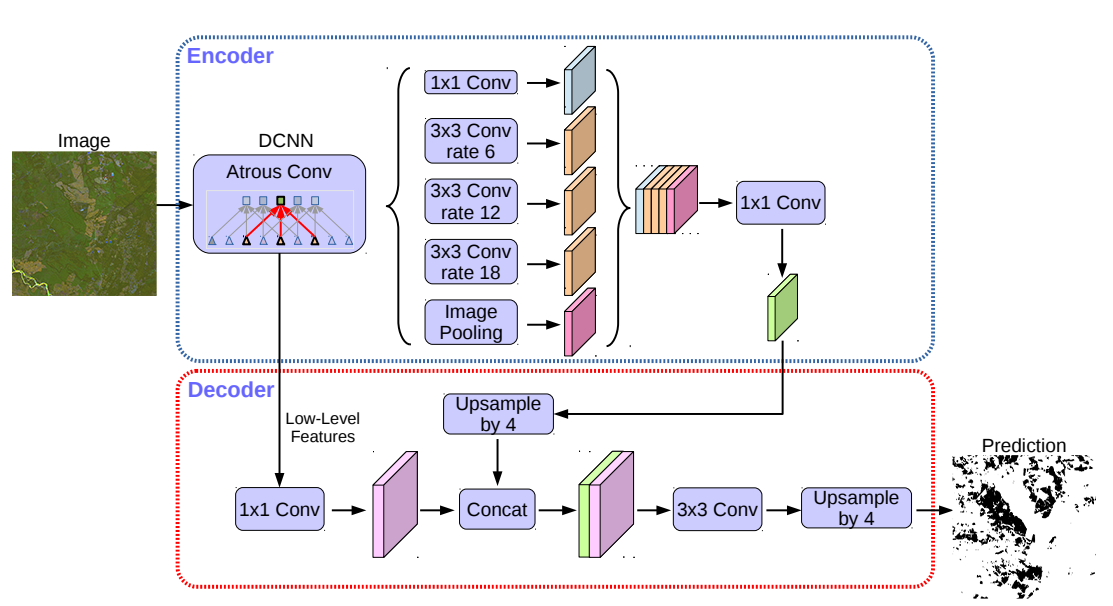
\includegraphics[width=\columnwidth]{model}
 \caption{Arquitectura DeepLabV3+ (Adaptado de \cite{chen2018})}
 \label{fig:model}
\end{figure}

Como se mencionó previamente la arquitectura se basa en un codificador poderoso que utiliza convolución atrous, una técnica que ha sido heredada de su predecesor DeepLabV34. Un avance notable en DeepLabV3+ es la introducción de convoluciones atrous separables. Esta innovación se traduce en una reducción significativa en el número de cálculos necesarios para el procesamiento de imágenes, sin comprometer la eficacia del modelo. Esta optimización se logra descomponiendo las convoluciones en dos partes: una convolución atrous seguida de una convolución punto a punto (1x1), lo que mejora tanto la eficiencia del cálculo como la precisión de la segmentación.

Por otra parte, el decodificador en DeepLabV3+ juega un papel fundamental en la mejora de la precisión de la segmentación, especialmente en los límites de los objetos. Trabaja para recuperar la información espacial que se pierde durante el proceso de codificación, asegurando así que los detalles finos y las fronteras de los objetos se capturen con precisión. Esta capacidad de refinamiento es lo que diferencia a DeepLabV3+ de otros modelos, permitiéndole producir resultados de segmentación más precisos y detallados.  La aplicación de convoluciones separables en profundidad tanto en el módulo ASPP como en el decodificador no solo mejora la precisión, sino que también aumenta la eficiencia computacional del modelo \cite{chen2018}.

Además, DeepLab a menudo incluye pasos adicionales para mejorar la precisión en los límites de los objetos. Esto se logra mediante la aplicación de técnicas avanzadas en la etapa de decodificación, asegurando que las fronteras de los objetos se mantengan nítidas y bien definidas. El resultado final es una predicción de píxeles altamente precisa, donde cada píxel en la imagen se asigna a una categoría específica, resultando en una segmentación detallada y precisa.

Otro aspecto importante de las redes backbone en DeepLabV3+ es su adaptabilidad a diferentes resoluciones de entrada. Esto permite que el modelo se ajuste a diferentes presupuestos de recursos computacionales, lo que es crucial en aplicaciones donde se necesita un equilibrio entre precisión y eficiencia. La capacidad de trabajar con diversas resoluciones asegura que DeepLabV3+ sea aplicable en una amplia gama de escenarios, desde dispositivos móviles con recursos limitados hasta potentes servidores de cómputo.

Finalmente, la integración de la red backbone con el módulo del decodificador en DeepLabV3+ es un factor clave para su éxito. Mientras que la red backbone actúa como un codificador, el módulo del decodificador refina los resultados de segmentación. Este refinamiento es especialmente crucial a lo largo de los límites de los objetos, donde el decodificador utiliza características de bajo nivel de la red backbone para mejorar la precisión. Además, el modelo utiliza convoluciones separables atrous en ambos módulos, ASPP y decodificador, para mejorar la eficiencia computacional sin sacrificar el rendimiento.
